\section{Постановка задачи}

Для исследования нам даны данные о покупках товаров одной категории за 2017--начало 2018 годы. Данные хранятся в отношении с заголовком:
\begin{center}
        (Код товара, Дата покупки, Количество),
\end{center}
причем в одну дату может быть быть совершено более одной покупки.

Мы будем исследовать совокупный спрос на все товары данной группы. Будем пользоваться СУБД \textit{MySQL} для быстрого доступа к данным и средствами модулей \textit{Python3} для их обработки, построения моделей и построения графиков. Визуализация совокупных покупок всех товаров, представленных в 2017 и 2018 годах, доступные для разработки алгоритма представлены на рисунке Рис.~\ref{img:data}.

\begin{figure}[h]
        \noindent\centering{
        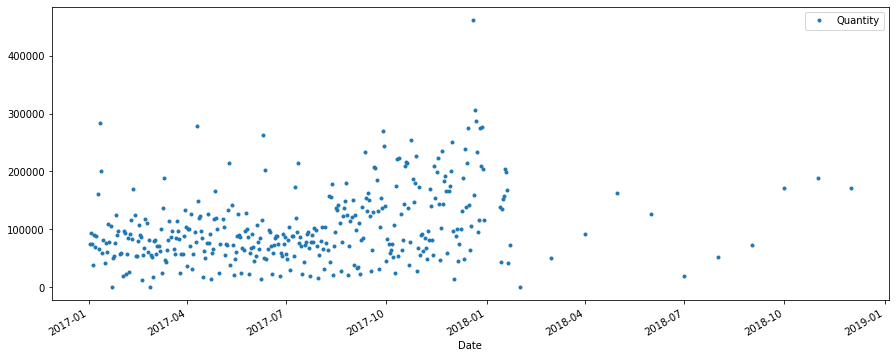
\includegraphics[width=160mm]{content/formulation/data.png}
        }
        \caption{Совокупные покупки по дням.}
        \label{img:data}
\end{figure}

Из рисунка видно, что данные за 2018 год не полные, поэтому мы сформулируем задачу следующим образом: 
\textit{Будем предсказывать дневной спрос в декабре 2017 года по считающемуся известным спросу за предыдущие месяцы.}